\documentclass[11pt]{article}

\usepackage[utf8]{inputenc}
\usepackage{indentfirst}
\usepackage{natbib}
\usepackage{graphicx}

\renewcommand{\contentsname}{Índice}

\begin{document}

\begin{titlepage}
   \begin{center}
       
       
\includegraphics[width=0.3\textwidth]{images/EscolaEngenhariaUM.jpeg}
       
       \vspace*{0.5cm}
       
       \textbf{\Large Sistema de gestão de stocks de um	armazém de uma fábrica}

       \vspace{1.3cm}
       \textbf{\large Desenvolvimento de Sistemas de Software - Grupo 10}
            
       \vspace{1.3cm}

       Bruno Filipe de Sousa Dias A89583\\ Guilherme Santiago Lopes Pereira A89479 \\ Luís Enes Sousa A89597\\ Pedro Miguel de Soveral Pacheco Barbosa A89529

       \vspace{1.5cm}
       
       
\includegraphics[width=35mm]{images/bruno.jpeg}\hspace{0.2cm}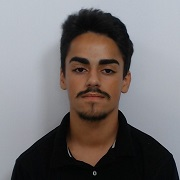
\includegraphics[width=35mm]{images/guilherme.jpeg}
       \vspace{0.15cm}
       \hspace{0.1cm}
\includegraphics[width=35mm]{images/luis.jpeg}\hspace{0.1cm}
\includegraphics[width=35mm]{images/pedro.jpeg}
       
        
        31 de outubro de 2020
            
   \end{center}
\end{titlepage}

\tableofcontents
\thispagestyle{empty}
\cleardoublepage

\setcounter{page}{1}

\section{Introdução}

Neste semestre, no âmbito da unidade curricular de Desenvolvimento de Sistemas de Software, foi-nos proposto o desenvolvimento de uma componente de um sistema de gestão de stocks de um armazém de uma fábrica de modo a pôr em prática toda a aprendizagem sobre Desenvolvimento de Sistemos de Software, com auxílio da linguagem de programação orientada aos objetos Java. O seu principal objetivo será desenvolver uma aplicação que suporte alguns cenários descritos no enunciado pelos docentes da cadeira e outros que serão definidos pelo nosso grupo consoante achemos pertinente ao longo da realização deste projeto.

O trabalho foi dividido em três fases de entrega sendo que a primeira consiste na análise de requisitos do projeto que será feita com base na conceção de um Modelo de Domínio e de um Modelo de Use Case com as funcionalidades propostas.

\section{Modelo de Domínio}

Para a aplicação que nos foi proposta desenvolvemos o Modelo de Domínio que se apresenta de seguida:

\begin{center}
    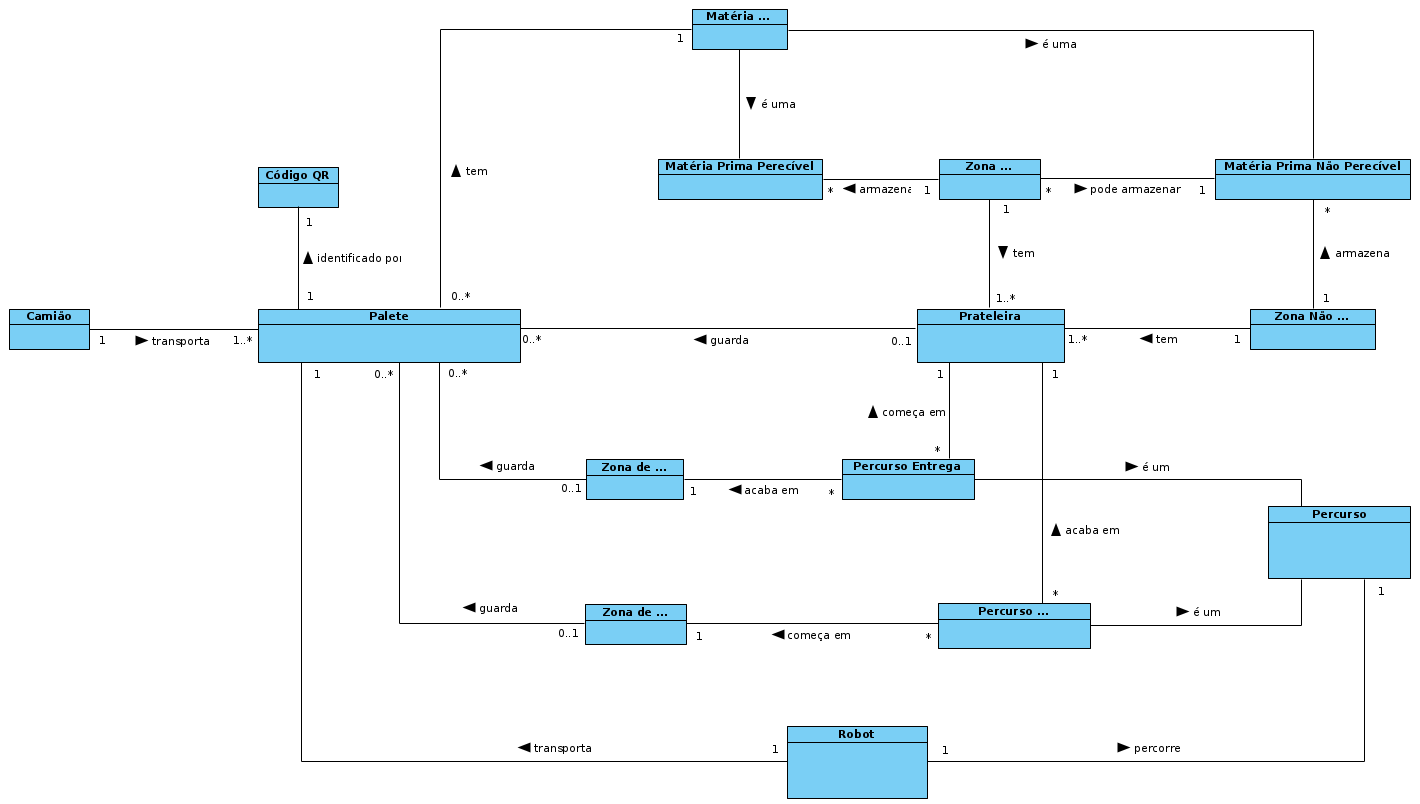
\includegraphics[width=150mm]{images/modelo de dominio.png}
\end{center}

Através da análise do Modelo de Domínio é possível tanto perceber quais as entidades relevantes no nosso projeto bem como as relações que as mesmas estabelecem entre elas. Deste modo, torna-se percetível a abordagem do nosso grupo para gerir o stock do armazém de uma fábrica. 

\section{Modelo de Use Case}

No decorrer da leitura do enunciado o nosso grupo conseguiu identificar 10 Use Cases e 6 atores. Os 6 atores são o camião que solicita autorização de descarga e descarrega o seu conteúdo ou fica à espera no queue para descarregar, o Gestor que autoriza os pedidos de descarga e controla a queue dos camiões e que solicita listagem com a localização das paletes no armazém, o Leitor de Códigos QR que lê os códigos das paletes, o Robot que recolhe as paletes, arruma-as e entrega-as notificando que o fez com sucesso, o Servidor de Produção que faz requisição do material necessário e o Encarregado que notifica o Sistema que as paletes lhe foram entregues com sucesso. Assim sendo, o nosso Modelo de Use Cases é o apresentado a seguir:

\begin{center}
    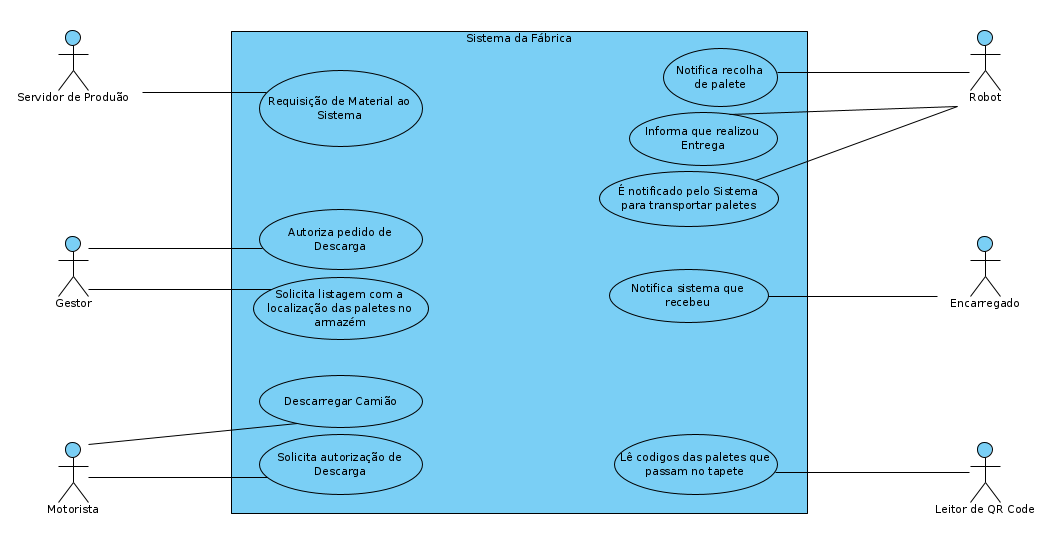
\includegraphics[width=150mm]{images/Use case.png}
\end{center}

\subsection{Use Case: Solicitar Autorização de Descarga}

\textbf{Descrição:} Camião chega à fábrica e solicita autorização para entrar na zona de receção para descarregar as paletes

\textbf{Ator:} Camião

\textbf{Cenários:} 1

\textbf{Pré-Condição:} True

\textbf{Pós-Condição:} Gestor é informado do pedido de descarga

\textbf{Fluxo Normal:}\\
        1. Camião solicita autorização de descarga\\
        2. Sistema informa gestor que um camião pretende descarregar
        
\textbf{Fluxo Alternativo: [gestor encontra-se ocupado a gerir outro pedido] (passo 2)}\\
        2.1. Sistema informa camião que gestor se encontra ocupado\\
        2.2. Camião aguarda que gestor fique livre\\
        2.3. Sistema informa gestor que um camião pretende descarregar
        
\textbf{Fluxo Excepcional: [camião desista da descarga] (passo 2.2)}\\
        2.2.1 Camião informa o sistema que não pretende efetuar a descarga


\vspace{3cm}


\subsection{Use Case: Autorizar pedido de Descarga}

\textbf{Descrição:} Gestor autoriza o pedido de Descarga por parte do camião

\textbf{Ator:} Gestor

\textbf{Cenários:} 1

\textbf{Pré-Condição:} Gestor recebeu um pedido de descarga

\textbf{Pós-Condição:} Camião entra na zona de receção

\textbf{Fluxo Normal:}\\
        1. Sistema informa gestor que um camião pretende descarregar\\
	    2. Gestor informa que a zona de receção se encontra livre\\
	    3. Gestor autoriza a descarga do camião\\
	    4. Camião entra na zona de receção para descarregar
        
\textbf{Fluxo Alternativo 1: [zona de receção encontra-se ocupada] (passo 2)}\\
        2.1. Gestor informa camião que zona de receção se encontra ocupada\\
	    2.2. Camião espera que zona de receção fique livre\\
	    2.3. Regressa a 3
        
\textbf{Fluxo Excepcional 1: [camião decide não descarregar] (passo 2.2)}\\
        2.2.1. Camião informa gestor que não pretende esperar para descarregar\\
	    2.2.2. Camião não entra na zona de receção e vai embora
	    
	    
\vspace{3cm}	    
	    
	    
\subsection{Use Case: Descarregar camião}

\textbf{Descrição:} Camião descarrega para a zona de armazém

\textbf{Ator:} Camião

\textbf{Cenários:} 1

\textbf{Pré-Condição:} Gestor aceitou o pedido de descarga do camião

\textbf{Pós-Condição:} Camião descarrega paletes

\textbf{Fluxo Normal:}\\
        1. Camião informa Sistema que pretende descarregar\\
    	2. Gestor verifica se existe espaço suficiente no armazém\\
	    3. Camião descarrega todas as paletes
        
\textbf{Fluxo Alternativo 1: [não existe espaço suficiente para todas as paletes] (passo 3)}\\
        3.1. Sistema informa camião que não existe espaço suficiente para todas as paletes\\
	    3.2. Camião descarrega paletes possíveis de armazenar\\
	    3.3. Regressa a 1
        
\textbf{Fluxo Excepcional 1: [camião decide não descarregar] (passo 3.2)}\\
        3.2.1. Camião informa Gestor que não pretende descarregar\\
	    3.2.2. Camião não descarrega e vai embora


\vspace{3cm}


\subsection{Use Case: Ler códigos das paletes que passam no tapete}

\textbf{Descrição:} Leitor de códigos QR lê os códigos das paletes que passam no tapete

\textbf{Ator:} Leitor de códigos QR 

\textbf{Cenários:} 1

\textbf{Pré-Condição:} Camião efetuou descarga na zona de receção

\textbf{Pós-Condição:} Palete fica pronta para ser armazenada

\textbf{Fluxo Normal:}\\
        1. Leitor QR faz um scan na palete\\
	    2. Sistema confirma que código QR é válido\\
	    3. Sistema guarda informações sobre dimensões, código único de identificação e sobre o tipo de material contido na palete\\
	    4. Leitor QR insere informação sobre local onde a palete deve ser guardada\\
	    5. Sistema adiciona palete à queue de paletes a transportar para a zona de armazenamento
        
\textbf{Fluxo Alternativo 1: [Sistema rejeita Código QR pois este é inválido] (passo 2)}\\
        2.1. Leitor de Código QR comunica que código QR é inválido\\
	    2.2. Sistema atribui novo código QR à palete\\
        2.3. Regressa a 3
   
   
\vspace{3cm}
   
        
\subsection{Use Case: Notificar Robot para Transporte de Palete}

\textbf{Descrição:} Sistema notifica robot para transportar palete

\textbf{Ator:} Robot

\textbf{Cenários:} 1

\textbf{Pré-Condição:} Palete encontra-se pronta para ser transportada

\textbf{Pós-Condição:} Robot é notificado para recolher Paletes

\textbf{Fluxo Normal:}\\
        1. Sistema escolhe Robot disponível com percurso mais eficiente (mais próximo)\\
        2. Sistema notifica Robot para transportar palete\\
        3. Robot recebe a notificação de que tem de transportar palete especificada

        
\textbf{Fluxo Alternativo 1: [não existe robots disponíveis no armazém] (Passo 1)}\\
        1.1. Sistema aguarda que um Robot fique disponível\\
        1.2. Regressa a 2
   
   
\vspace{3cm} 
   
        
\subsection{Use Case: Notificar Recolha da Palete}

\textbf{Descrição:} Robot notifica Sistema que recolheu palete

\textbf{Ator:} Robot

\textbf{Cenários:} 1

\textbf{Pré-Condição:} Robot foi notificado para recolher palete

\textbf{Pós-Condição:} Palete é recolhida

\textbf{Fluxo Normal:}\\
        1. Robot recolhe palete pedida na sua tarefa\\
	    2. Robot notifica o Sistema que recolheu palete pedida\\
	    3. Sistema remove palete da queue de paletes a ser transportadas


\vspace{3cm}

	    
\subsection{Use Case: Informar que realizou Entrega com sucesso}

\textbf{Descrição:} Robot informa que realizou a entrega de uma palete com sucesso

\textbf{Ator:} Robot

\textbf{Cenários:} 1

\textbf{Pré-Condição:} Robot realizou entrega de uma palete

\textbf{Pós-Condição:} Sistema é notificado com sucesso

\textbf{Fluxo Normal:}\\
        1. Robot notifica o Sistema que entregou palete com sucesso\\
	    2. Sistema regista que palete foi entregue pelo Robot


\vspace{4cm}


\subsection{Use Case: Fazer requisição de material}

\textbf{Descrição:} Servidor da Produção faz uma requisição de material ao Sistema

\textbf{Ator:} Servidor da Produção

\textbf{Cenários:} 2

\textbf{Pré-Condição:} True

\textbf{Pós-Condição:} Paletes requisitadas ficam registadas na queue de paletes a ser transportadas

\textbf{Fluxo Normal:}\\
        1. Servidor da Produção requisita materiais\\
    	2. Sistema seleciona paletes para satisfazer requisição\\
    	3. Sistema regista paletes na queue de paletes a ser transportadas
        
\textbf{Fluxo Excecional 1: [não existem todas as paletes necessárias para satisfazer requisição] (Passo 2)}\\
        2.1. Sistema propõe ao Servidor da Produção entrega apenas dos materiais existentes\\
    	2.2. Servidor da Produção aceita proposta do Sistema\\
    	2.3. Sistema regista paletes existentes na queue de paletes a ser transportadas\\
    	2.4. Sistema regista paletes em falta na queue de paletes em falta
        
\textbf{Fluxo Excecional 2: [Servidor da Produção rejeita proposta do Sistema] (Passo 2.2)}\\
        2.2.1. Servidor de Produção rejeita proposta do Sistema\\
        2.2.2. Sistema cancela requisição
        
        
\vspace{3cm}

	    
\subsection{Use Case: Notificar satisfação de requisição}

\textbf{Descrição:} Encarregado notifica Sistema que as paletes lhe foram entregues

\textbf{Ator:} Encarregado

\textbf{Cenários:} 2

\textbf{Pré-Condição:} Paletes chegaram à zona de Entregas

\textbf{Pós-Condição:} Sistema regista paletes que chegaram à zona de Entregas

\textbf{Fluxo Normal:}\\
        1. Encarregado notifica o sistema que paletes chegaram à zona de Entregas\\
        2. Sistema regista paletes que chegaram à zona de Entregas
        
    
\vspace{3cm}

	    
\subsection{Use Case: Solicitar listagem com a localização das paletes no armazém}

\textbf{Descrição:} Gestor solicita a listagem com a localização de todas as paletes no armazém

\textbf{Ator:} Gestor

\textbf{Cenários:} 3

\textbf{Pré-Condição:} True

\textbf{Pós-Condição:} Sistema entrega listagem completa 

\textbf{Fluxo Normal:}\\
        1. Gestor pede listagem com a localização de todas as paletes no armazém\\
        2. Sistema recolhe dados de todas as paletes no armazém\\
        3. Sistema entrega listagem da localização de todas as paletes no armazém ao Gestor

\textbf{Fluxo Excecional 1: [Sistema não consegue recolher dados] (Passo 2)}\\
        2.1. Sistema não recebe dados necessários para formar a lista pedida\\
        2.2. Gestor não recebe lista de localização das paletes pedida

\vspace{2.5cm}
	    
\section{Conclusão}

Concluindo, nesta fase do projeto foi-nos pedido a análise de requisitos do projeto e prosseguimos à elaboração de dois Modelos o de Domínio e o de Use Cases. Todo este processo permitiu o grupo ter uma melhor perceção das entidades relevantes do projeto bem como as relações que estas estabelecem entre elas. Seguidamente, analisamos os requisitos funcionais do nosso projeto tentando perceber quais os atores intervenientes e quais as ações que estes iriam desempenhar no trabalho. Deste modo, pensamos que atingimos o nosso objetivo que consistia em perceber através da conceção dos modelos como é que iríamos gerir o stock do armazém da fábrica com principal foco tanto nas entidades existentes como na maneira como estas se vão relacionar entre si. Esperamos assim ter conseguido, através da elaboração da 1ª fase do projeto, ter construido uma boa base para construirmos uma aplicação o mais eficiente e completa possível.

\end{document}



